\documentclass{article}
\usepackage{tikz}
\usepackage[x11names, rgb]{xcolor}

\begin{document}
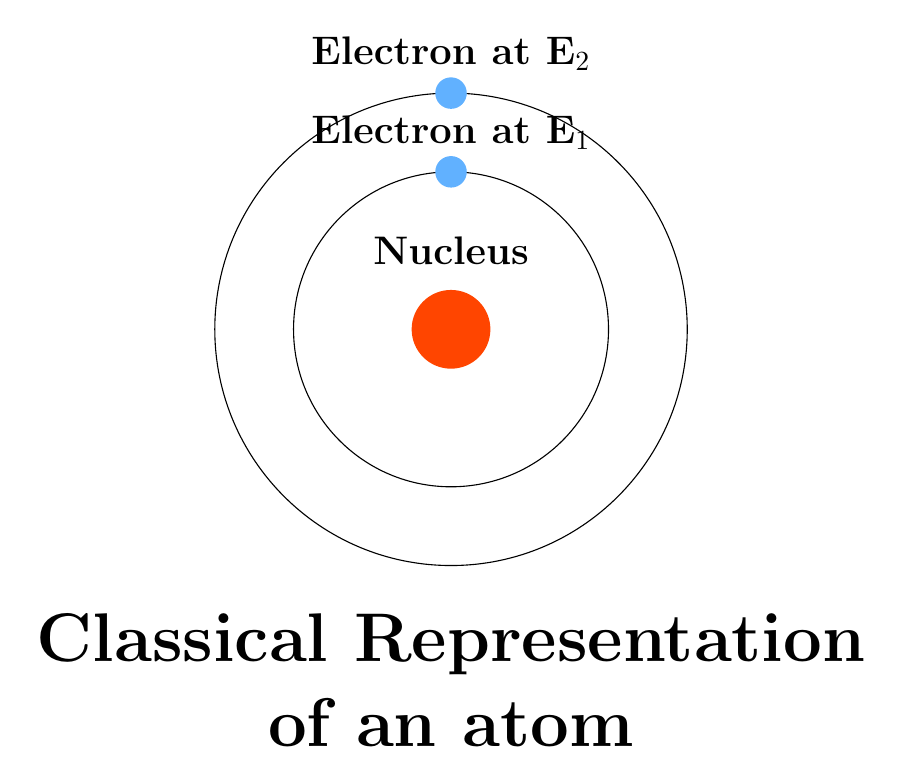
\begin{tikzpicture}

\draw (1,1) circle (2cm);
\draw (1,1) circle (3cm);

\definecolor{atom_blue}{HTML}{1E90FF}
\definecolor{atom_red}{HTML}{FF4500}

\fill[atom_red!100] (1,1) circle (.5cm);
\node at (1, 2) {\textbf{\Large Nucleus}};

\fill[atom_blue!70] (1,3) circle (.2cm);
\node at (1, 3.5) {\textbf{\Large Electron at E$_{1}$}};

\fill[atom_blue!70] (1,4) circle (.2cm);
\node at (1, 4.5) {\textbf{\Large Electron at E$_{2}$}};

\node at (1, -3) {\textbf{\Huge Classical Representation}};
\node at (1, -4) {\textbf{\Huge of an atom}};

\end{tikzpicture}
\end{document}
